% ONLY IN CHAPTER 1

\addtocontents{toc}{\vspace{2em}} % Add a gap in the contents, for aesthetics

% Begin numeric (1,2,3...) page numbering

\pagestyle{fancy} % Return the page headers back to the "fancy" style

% Chapter 1

\chapter{Introduction} % Main chapter title

\label{chap:ntroduction} % For referencing the chapter elsewhere, use \ref{Chapter1} 

\lhead{Chapter 1. \emph{Introduction}} % This is for the header on each page - perhaps a shortened title

%----------------------------------------------------------------------------------------

\section{Graphs and graph signals}

In the field of discrete mathematics, the term ``graph" denotes a collection of distinct objects that may possess some form of pairwise connection or association. The discrete objects that make up the graph are referred to as nodes (or vertices), and their connections are known as edges (or arcs). This abstract definition can be applied to represent numerous real-world structures. For example, in an airline route map, nodes could symbolise airports, and edges could indicate the presence of a direct flight.


\begin{wrapfigure}{r}{0.4\linewidth}
	\centering
		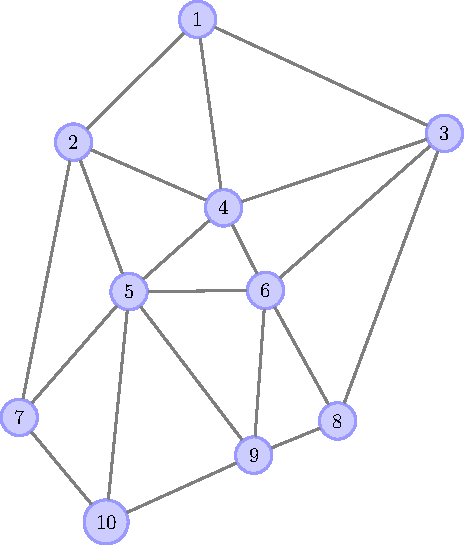
\includegraphics[width=\linewidth]{Figures/graph_plot.pdf}
	\caption[A visual representation of a simple graph]{A visual representation of a simple graph with 10 nodes and 20 edges.}
	\label{fig:basic_graph}
\end{wrapfigure}


Graphs and network models are employed in many actively researched areas of mathematics, including network processes such as epidemic modelling \citep{Pare2020}, graph neural networks \citep{Zhou2020}, graphical models \citep{Holmes2008}, and semi-supervised learning \citep{Chong2020}.

In this thesis, we focus primarily on the area of Graph Signal Processing (GSP), a rapidly evolving field that sits at the intersection of spectral graph theory, statistics, and data science \citep{Ortega2018}. GSP is devoted to the mathematical analysis of signals that are defined over the nodes of a graph, simply referred to as \textit{graph signals}. \phantom{In this thesis we are  }

\begin{wrapfigure}{l}{0.4\linewidth}
	\centering
		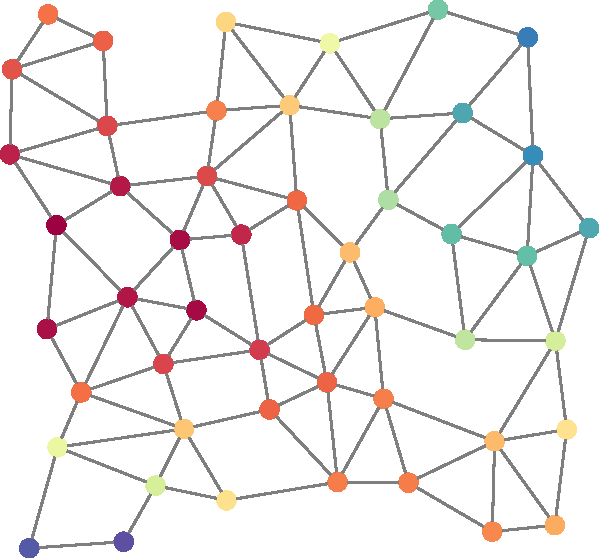
\includegraphics[width=\linewidth]{Figures/graph_signal_plot.pdf}
	\caption[A graphical depiction of a graph signal]{A graphical depiction of a graph signal. Here, the value of the signal at each node is represented by its color.}
	\label{fig:graph_signal}
\end{wrapfigure}
 

A graph signal represents a value that is measured simultaneously at every node in a graph. For example, consider a social media network, where each node represents an individual, and presence of an edge indicates that the two individuals have connected. An example of a graph signal in this context could be the age of each person in the network, or a score indicating their propensity to engage with certain content. In either case, this is a value that could theoretically be measured or estimated across the network, though it may be subject to missing data or noise. 

GSP typically uses tools that stem from classical signal processing. There, the focus is on manipulating data that resides on a regular domain, such as audio, images and digital communication. GSP utilises spectral graph theory to generalise these classical techniques, leading to graph-based counterparts of algorithms such as filtering, sampling, and reconstruction \citep{Shuman2013, Sandryhaila2013}. Applications of GSP are numerous, ranging from social networks \citep{Dong2015} and brain connectivity modelling \citep{Huang2016} to sensor networks \citep{Zhu2012}, and molecular structures \citep{Kearnes2016}. As an emerging field, there are many opportunities for the development of theory, and new use-cases to explore, making it an exciting and dynamic area of research. 

The primary focus of this thesis is on statistical models for the estimation of noisy, partially observed multivariate graph signals. In particular, we formulate several Bayesian regression and reconstruction models designed for multivariate data, and investigate scalable approaches to solving them in practice. This begins, in \cref{chap:gsr_2d}, with the reconstruction of signals with two axes, such as network time series data. \Cref{chap:kgr_rnc_2d} introduces several regression techniques for two-dimensional graph signals, and \cref{chap:nd_gsp} generalises the techniques developed prior in the thesis to $d$-dimensional data, under the ``Multiway" GSP (MGSP) framework. This is followed, in \cref{chap:variance}, by an investigation into the posterior covariance of the models, and finally \cref{chap:binary} introduces generalisations for binary and categorical graph signals. Along the way, there are several methodological contributions as well as some detailed case studies. In this introductory chapter, we first establish some basic definitions and concepts from GSP, as well as highlighting some motivating use cases. In \cref{chap:lit_review}, we define the precise scope of this thesis, review the relevant literature, and present our core contributions. 


\section{GSP fundamentals}

A graph, $\mathcal{G}$, with $N$ vertices is described by a node set $\mathcal{V}$, and an edge set $\mathcal{E}$. In this thesis, we will be primarily concerned with undirected graphs without self-loops, meaning the edges have no preferential direction and nodes do not connect to themselves. By imposing some arbitrary but consistent ordering on the nodes, this graph can also be described by an $N \times N$ adjacency matrix $\A$, where the entry $\A_{ij} = \A_{ji} \geq 0$ holds the strength of connection between nodes $i$ and $j$. In the basic case of a non-weighted graph, $\A_{ij}$ is simply one if the corresponding edge exists and zero otherwise. Using the same ordering, a graph signal can be represented by a vector, $\y$, of length $N$, where $\y_i$ holds the value of the graph signal at node $i$. 

One key property of a graph signal is its \textit{smoothness}. Intuitively speaking, a smooth graph signal should have gentle variation between closely connected nodes, as is the case in \cref{fig:graph_signal}. Conversely, a rough graph signal might see large jumps in signal value between neighbouring nodes. Mathematically, the smoothness of a signal, $\y$, defined over the nodes of an undirected graph, can be measured in several ways. One simple option is the Total Square Variation (TSV), defined as follows. 

\begin{equation}
    \label{eq:TSV1}
    \text{TSV}(\y) = \frac{1}{2}\sum_{i, j} \A_{ij} (\y_i - \y_j)^2
\end{equation}

This measure sums up the square difference in signal value at each neighbouring node, weighted by the corresponding entry in the adjacency matrix, with the factor of a half adjusting for the double counting of nodes. This expression can also be written in terms of a single quadratic form, by introducing a new matrix $\LL$ - the so-called graph \textit{Laplacian}. 

\begin{equation}
    \label{eq:TSV2}
    \text{TSV}(\y) = \y^\top \LL \y
\end{equation}

The Laplacian, $\LL$, is another symmetric $N \times N$ matrix, and is defined as $\LL = \D - \A$, where $\D$ is the degree matrix. $\D$ is diagonal, where entry $\D_{ii}$ holds the sum of all the edge weights linked to node $i$, or in other words, the vector along the diagonal of $\D$ is the column (or row) sum of $\A$. It is straightforward to show that the two expressions for the total square variation given in \cref{eq:TSV1,eq:TSV2} are equivalent, see for example chapter 3 of \cite{Ortega2022}. 

\newpage

A few basic facts stand out about the Laplacian quadratic form.

\begin{enumerate}
    \item $\y^\top \LL \y \geq 0$ for any $\y$. Since $\text{TSV}(\y)$ sums the square difference between the signal at each pair of nodes, weighted by the non-negative entries of the adjacency matrix, the Laplacian quadratic form must be strictly non-negative. By definition, this implies that the matrix $\LL$ is positive semi-definite (PSD). 
    \item $\one^\top \LL \one = 0$, where $\one$ is a length-$N$ vector of ones. If the signal of interest is constant over the whole graph, the total square variation must be zero. Furthermore, if the graph contains two or more isolated sub-graphs, with edges connecting nodes within a each group but not between groups, then any signal that is constant over each sub-graph will have a Laplacian quadratic form of zero. 
\end{enumerate}

Since $\LL$ is positive semi-definite, its eigenvalues are all real and non-negative, and its eigenvectors can be chosen to be real and orthonormal. Thus, $\LL$ can be decomposed as 

\begin{equation}
    \LL = \U \LAM \U^\top
\end{equation}

where $\U$ is the square, $N \times N$ matrix of orthogonal eigenvectors $\{\uu_i\}$, and $\LAM$ is the diagonal matrix of eigenvalues, typically listed in ascending order. 

\begin{equation*}
    \U = \begin{bmatrix}
        \vertbar{4.5}{0.5}{-3} & \vertbar{4.5}{0.5}{-3} & & \vertbar{4.5}{0.5}{-3} \\
        \uu_1    & \uu_2    & \ldots & \uu_N    \\
        \vertbar{4.5}{0.5}{0.5} & \vertbar{4.5}{0.5}{0.5} & & \vertbar{4.5}{0.5}{0.5} 
    \end{bmatrix}, \quad\quad\quad \LAM = \begin{bmatrix}
        \lambda_1 & & & \\
        & \lambda_2 & & \\
        & & \ddots & \\
        & & & \lambda_N
    \end{bmatrix}
\end{equation*}

Since $\U$ is orthonormal, it holds that $\uu_i^\top \uu_j = \delta_{ij}$, and that $\{\uu_i\}$ form a set spanning $\R^N$. Given the definition of the Laplacian quadratic form, the eigenvectors are the orthonormal set of vectors that sequentially minimise the total square variation, subject to perpendicularity to all those previous. 

$$
\begin{matrix}
    \uu_1 & = & \underset{|\uu|^2 = 1}{\text{argmin}} \quad & \text{TSV}(\uu) \\[0.5cm]
    \uu_2 & = & \underset{|\uu|^2 = 1, \perp \uu_1}{\text{argmin}} \quad & \text{TSV}(\uu) \\[0.5cm]
    \uu_3 & = & \underset{|\uu|^2 = 1, \perp \uu_1, \uu_2}{\text{argmin}} \quad & \text{TSV}(\uu) \\[0.5cm]
    & & \vdots & 
\end{matrix}
$$

In this way, the eigenvectors of the graph Laplacian can be understood as sequentially less and less smooth, with respect to the topology of the graph. The corresponding eigenvalue, often referred to as the frequency, gives a value specifying how ``rough'' each eigenvector is relative to the others. Note that, for any undirected graph, the first Laplacian eigenvector will always be constant with an eigenvalue of zero. \Cref{fig:cali_eigs} gives a visual depiction of the first nine Laplacian eigenvectors and eigenvalues for a network representing regions in California. 

\begin{figure}[t]
	\centering
		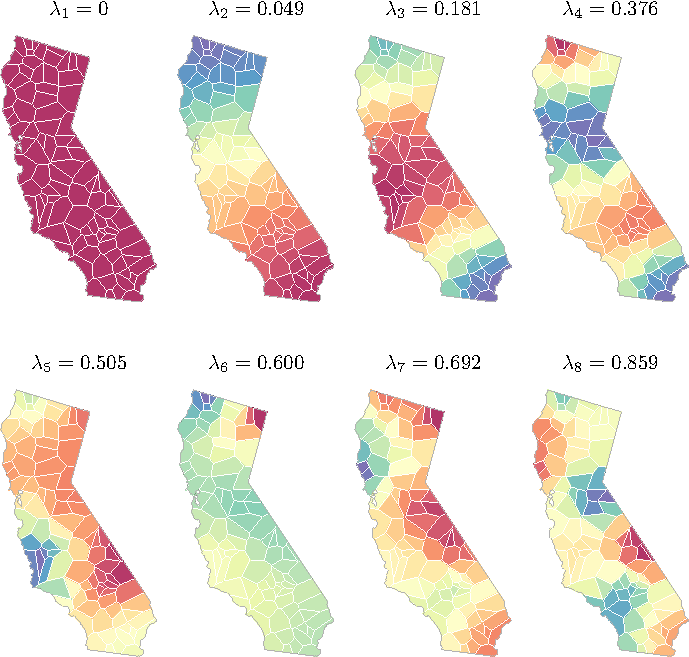
\includegraphics[width=0.85\linewidth]{Figures/cali_plot_eigs.pdf}
	\caption[A visualisation of the Laplacian eigenvectors for a network of regions in California]{A visualisation of the first nine Laplacian eigenvectors, along with their associated eigenvalue, for a network of regions in California. Each node represents a region, and each pair or regions share an edge if they border one another. Again, color is used to represent the value of the the graph signal. }
	\label{fig:cali_eigs}
\end{figure}


  
% \begin{figure}[t]
% 	\centering
% 		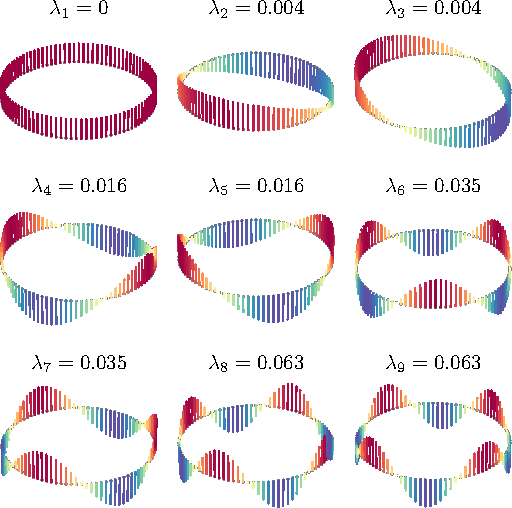
\includegraphics[width=0.7\linewidth]{Figures/loop_plot.pdf}
% 		% \rule{35em}{0.5pt}
% 	\caption[Eigenvectors of the loop graph Laplacian]{A graphical depiction of the eigenvectors of the loop graph Laplacian.  }
% 	\label{fig:loop_plot}
% \end{figure}
 

Since $\{\uu_i\}$ span the total space of $\R^N$, any graph signal $\y$ can be decomposed into a weighted sum of the Laplacian eigenvectors. This has a direct analogy with classical signal processing, where a 1D signal on a regular domain can be broken into its frequency components via the Fourier transform. 

\begin{equation}
    \y = \sum_{i=1}^N z_i \uu_i 
\end{equation}

As such, any graph signal, $\y$, has a duel representation, $\z$, in the Laplacian frequency space. Transformations between these two representations can be achieved by applying the Graph Fourier Transform (GFT) and Inverse Graph Fourier Transform (IGFT), which amounts to multiplying by the matrices $\U^\top$ and $\U$ respectively. 

\begin{align}
    \z &= \text{GFT}(\y) = \U^\top \y \\[0.2cm]
    \y &= \text{IGFT}(\z)  = \U \z
\end{align}






\section{Some motivating examples}

Graphs and graph signals have proven a useful way to describe data across a broad range of applications owing to their flexibility and relative simplicity. They are able to summarise the of key properties large, complex systems within a single easily-digestible structure. Much of the data encountered in modern applications can be wel-described by a graph, evidenced by the rise of graph databases such as Neo4j \citep{Webber2012}. 


\section{Thesis overview}

\label{sec:thesis_overview}